%%%%%%%%%%%%%%%%%%%% author.tex %%%%%%%%%%%%%%%%%%%%%%%%%%%%%%%%%%%
%
% Template for the Handbook of Gravitational Wave Astronomy
%
%%%%%%%%%%%%%%%% Springer %%%%%%%%%%%%%%%%%%%%%%%%%%%%%%%%%%
\documentclass[graybox, nosecnum]{svmult}

% choose options for [] as required from the list
% in the Reference Guide

\usepackage{mathptmx}       % selects Times Roman as basic font
\usepackage{helvet}         % selects Helvetica as sans-serif font
\usepackage{courier}        % selects Courier as typewriter font
\usepackage{type1cm}        % activate if the above 3 fonts are
                            % not available on your system
 \usepackage{verbatim}
%
\usepackage{makeidx}         % allows index generation
\usepackage{graphicx}        % standard LaTeX graphics tool
                             % when including figure files
\usepackage{multicol}        % used for the two-column index
\usepackage[bottom]{footmisc}% places footnotes at page bottom
\usepackage{hyperref}        %for hyperlinks
\usepackage{soul}            % for high-lighting of text
\usepackage[dvipsnames]{xcolor}
\hypersetup{colorlinks=true,urlcolor=blue}
%
\usepackage[square,numbers]{natbib}
%\bibliographystyle{ieeetr} 
\newcommand{\hbindex}[1]{\hl{#1}\index{#1}}  %highlights index entries
\makeindex             % used for the subject index
                       % please use the style svind.ist with
                       % your makeindex program
%%%%%%%%%%%%%%%%%%%%%%%%%%%%%%%%%%%%%%%%%%%%%%%%%%%%%%%%%%%%%%%%%%%%%%%%%%%%%%%%%%%%%%%%%

\begin{document}
%\tableofcontents{}
\title*{3rd Generation Gravitational Wave Observatories}
% Use \titlerunning{Short Title} for an abbreviated version of
% your contribution title if the original one is too long
\author{Harald Lück \thanks{corresponding author}, Joshua Smith and Michele Punturo}
% Use \authorrunning{Short Title} for an abbreviated version of
% your contribution title if the original one is too long
\institute{Harald Lück \at Institut für Gravitationsphysik, Leibniz Universität Hannover and Max-Planck Institut für Gravitationspyhsik, Max-Planck Gesellschaft, Germany , \email{harald.lueck@aei.mpg.de}
\and Michele Punturo \at Istituto Nazionale di Fisica Nucleare Perugia, Perugia, Italy, \email{michele.punturo@pg.infn.it}
\and Joshua R. Smith \at Nicholas and Lee Begovich Center for Gravitational-Wave Physics and Astronomy, California State University, Fullerton, US, \email{josmith@fullerton.edu}
}
%
% Use the package "url.sty" to avoid
% problems with special characters
% used in your e-mail or web address
%
\maketitle
%
\abstract{
The second generation of gravitational-wave detectors has opened a new window on the cosmos, yet leaves much of the gravitational universe unexplored. 
A greatly more sensitive third generation of observatories is currently being planned: The Einstein Telescope in Europe and Cosmic Explorer in the US. 
The Einstein Telescope is envisaged as an underground observatory in the shape of an equilateral triangle with a side length of 10\,km located in Europe. Cosmic Explorer, on the other hand, aims for an above-ground L-shaped detector with up to 40\,km long arms in the US. These detectors will be capable of observing the post-merger phase of neutron star mergers, measuring every stellar mass black hole and neutron star merger in the universe -- including some with incredible precision, and of mapping the stellar evolution of the universe. 
These projects are currently in the design stage and are expected to start operations around the mid-thirties. The concepts are slightly different, but have many technical similarities.}
\section{Keywords} 
Einstein Telescope, Cosmic Explorer, Voyager, NEMO, third generation, 3G

\section{Introduction}

% The scientific field of 
Gravitational wave physics has experienced a rapid upswing following the historic first detection of gravitational waves (GW) from a pair of merging black holes (BH), GW150914, in 2015 by the two advanced LIGO detectors~\cite{aLIGO}. Further, the 2017 discovery by advanced LIGO and advanced Virgo of the binary neutron star merger GW170817 opened an era of multi-messenger gravitational-wave astronomy and received significant appreciation by the wider scientific community. 
% Not only the detection itself attracted extraordinary attention, but above all 
The scientific findings from the advanced LIGO and advanced Virgo observation runs completed to date (O1, O2 and O3) have inspired scientists by providing further insights into previously unexplored areas. In the first two observation runs in the period from 2015 to 2017 a total of 11 GW events were observed~\cite{GWTC1-2019}. Analysis of the first half of the third observation run (O3a, April 1st to October 1st, 2019) produced another 39 events from coalescing pairs of BH or a BH with a neutron star (NS)\cite{GWTC2-2020}. The second half of this observation run (O3b, November 1st, 2019 to March 27th 2020) is still being analysed with about two dozen more candidates.  

Despite the incredible sensitivity of these instruments and the impressive scientific results already obtained, the detection range and number of observations is still too small for 
% cosmological studies, 
deep explorations of the universe and the signal-to-noise ratio obtained comes mainly from the inspiral phase of coalescence of binary systems and is not yet sufficient to satisfactorily study the merger process and ring-down of the emerging new object. 
To exploit more of the potential of GW astronomy, the sensitivity of the detectors must be further increased. For the future it is planned to increase the sensitivity by one order of magnitude and over a wide frequency range beyond the design sensitivity of current detectors.  In parallel, the frequency range will be extended down to a few Hz in order to observe interesting sources emitting gravitational waves in this low-frequency band.
Gravitational wave astronomy is still in its infancy and just about to take the first steps.

For the next decade, the scientific program of the network of the LIGO, Virgo and KAGRA detectors foresees two more data taking periods (O4 in 2022-2023 and O5 in 2025-2026), alternating with periods of detector upgrades, until $\sim$2026\,-\,2027. During this period, the detector sensitivity will increase by up to a factor $\sim$3\,-\,5 for Virgo and $\sim3$ for LIGO, i.e. about a factor of two beyond their design sensitivities. The Japanese detector KAGRA joined the network in April 2020 and LIGO India, a third version of the advanced LIGO detectors currently being constructed in India, will become operational around 2026. Concrete plans for the period after 2027 have not yet been made. However, it is likely that upgraded versions of the three advanced LIGO detectors, advanced Virgo and KAGRA  (five detectors in total) will be operating until the end of the next decade. 

It became obvious quite early that the infrastructure of the LIGO and Virgo detectors built in the 1990s would offer only limited possibilities beyond these upgrades. The infrastructures themselves, with the necessary machinery, are neither designed nor suitable for the desired increase in sensitivity  {\color{green} (see also chapter 8)}. The planned retrofits of existing detectors within the next decade will push the limits of the infrastructures, both in terms of durability and performance, and therefore no significant further improvements in the existing infrastructures will be possible.
In the long run, any further increase in sensitivity can only be achieved by increasing the size of the detectors and building dedicated ultra-low noise infrastructures. Furthermore, the scientific community is quite keen to conduct regular and frequent data runs to obtain new data for continued new scientific discoveries. A radical reconstruction of the existing infrastructures would not only lead to considerable costs but also to unwanted downtime of the observatories and delays in the observation runs.

A third generation (3G) of instruments with significantly longer baselines and facility lifetimes of 50 years are currently being planned. Two leading 3G concepts have emerged: The Einstein Telescope in Europe and Cosmic Explorer in the US. The Einstein Telescope is envisaged as an underground observatory in the shape of an equilateral triangle with a side length of 10\,km located in Europe. Cosmic Explorer aims for an above-ground L-shaped detector with up to 40\,km long arms in the US.

At the time of writing (2020) we are in the fortunate position of having highly sensitive detectors capable of detecting gravitational waves at a rate of about one merger event per week. So far, these are all from binary star systems with black holes, neutron stars or other unknown objects. The signals have provided us with remarkable scientific results, but the capabilities of gravitational wave astronomy are far from exhausted; quite the contrary - the age of gravitational wave astronomy is just beginning. By peering more deeply into the gravitational universe we will observe a variety of sources and unlock a treasure of scientific results. 
Below we summarise the main scientific objectives that will be pursued with the next generation of gravitational wave detectors.

\section{3G Science Targets}

Following a study \cite{GWIC-SC} made by the Gravitational Wave International Committee (GWIC), the targets of the next generation of gravitational wave detectors can be grouped into the following topics:
\begin{quotation}

\begin{itemize}
\item explore new physics in gravity and in the fundamental properties of compact objects,
\item determine the properties of the hottest and densest matter in the Universe,
\item reveal the merging black hole population throughout the Universe and search for massive black
hole seeds,
\item understand the physical processes and mechanisms that underlie the most powerful astrophysical
phenomena,
\item investigate the particle physics of the primeval Universe and probe its dark sectors.
\end{itemize}

\end{quotation}

The immense scientific potential of a network of third-generation gravitational wave detectors is already evident in the enormous distance at which it can still observe compact merging binary systems. With the design sensitivities of the Einstein Telescope and CE2 as shown in figure~\ref{fig:2G-3G_curves}, binary systems of merging black holes can be observed up to a redshift of about 100 (see figure~\ref{fig:3Grange} and~\ref{fig:2G-3G_range}). This goes far beyond the distances at which electromagnetic telescopes can observe individual sources. The next generation of gravitational wave detectors offers a unique window on the earliest moments of structure formation in the universe. The following overview of science targets is based on the community's contribution to the GWIC 3G science case. More detail and thorough references can be found in that document~\cite{GWIC-SC}.   

\begin{comment}
\begin{figure}[htbp]
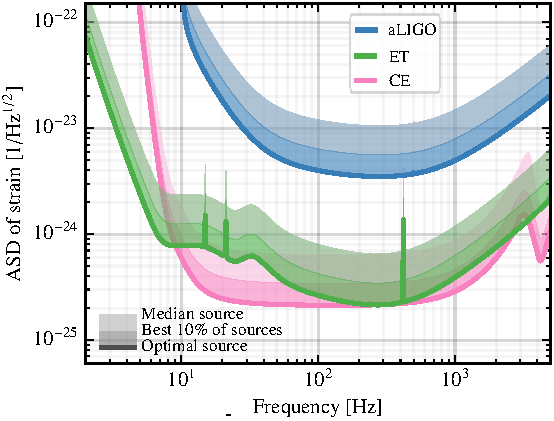
\includegraphics[width=0.8\textwidth]{Figures/noises_percentiles.pdf}
\caption{Target sensitivity curves for 3G gravitational-wave detectors ET, shown in green, and CE, shown in pink, compared with the design sensitivity of Advanced LIGO, shown in blue. 
The shades of the curves represent the sensitivity to sources with differently distributed sky locations and random inclination.}
\label{fig:3GSens}
\end{figure}
\end{comment}

\begin{figure}[htbp]
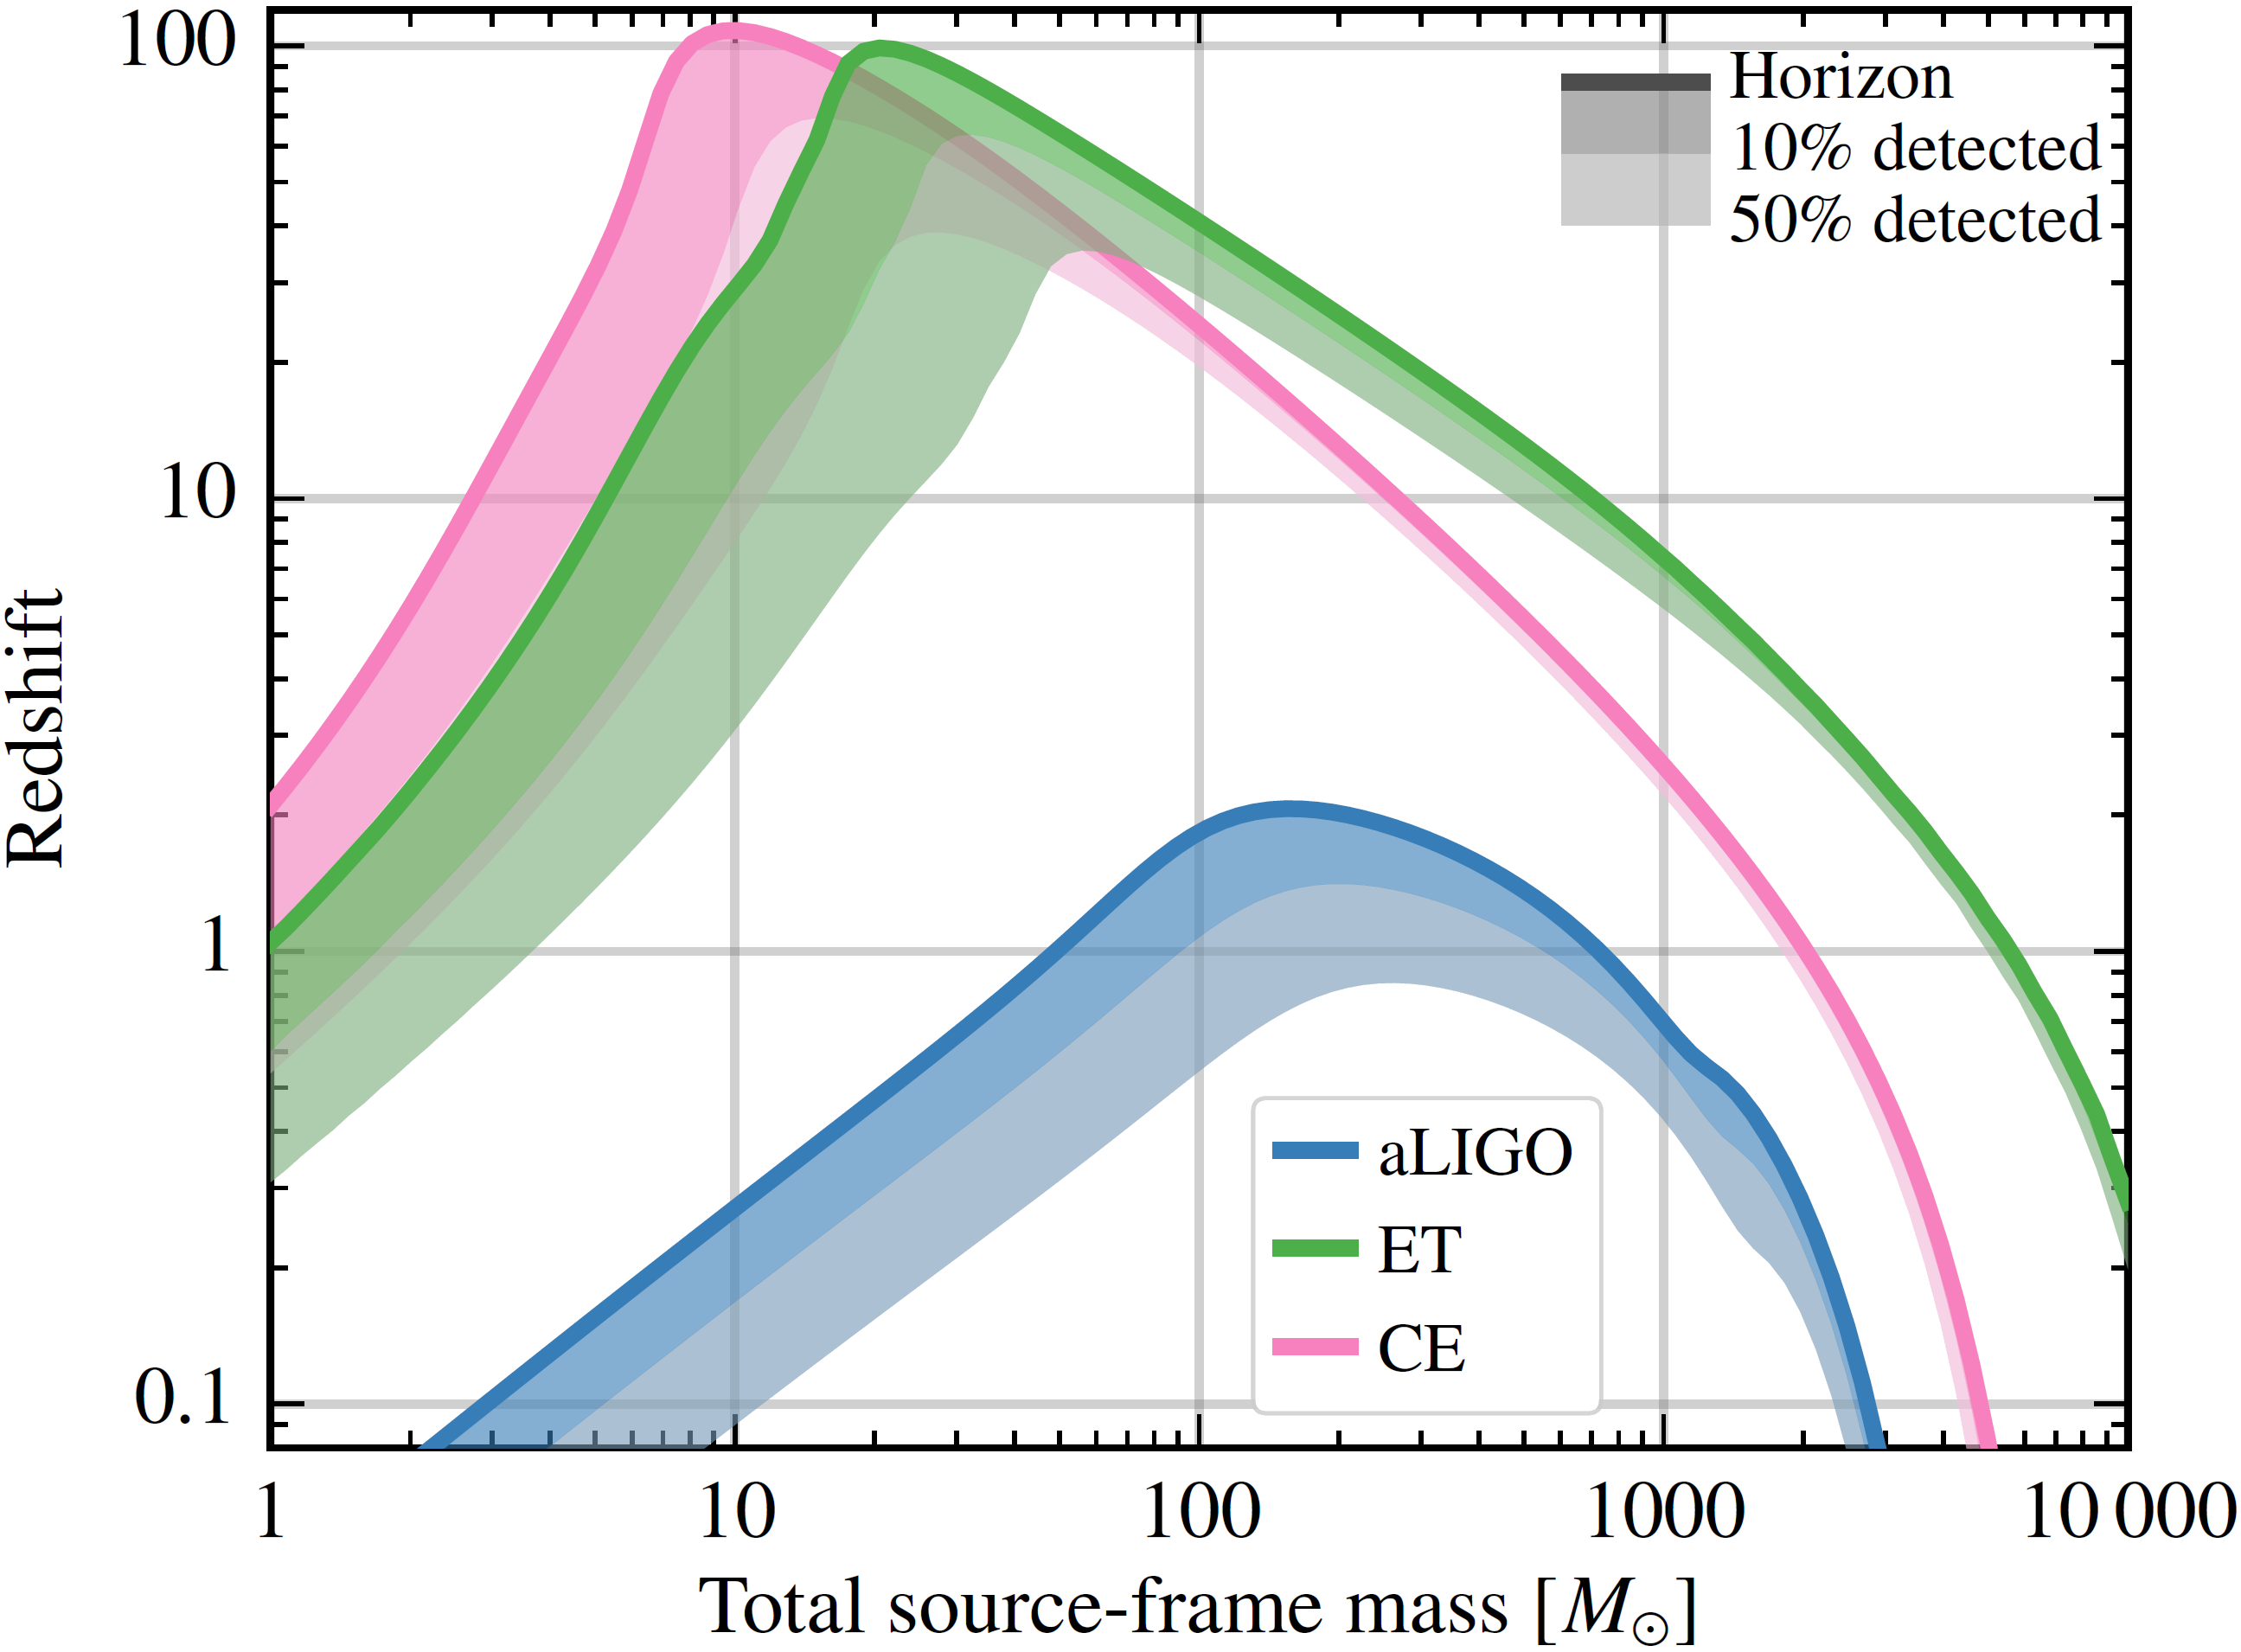
\includegraphics[width=0.8\textwidth]{Figures/InspiralRange.png}
\caption{Astrophysical reach for equal-mass, non-spinning binary systems. 
%Colours as in figure~\ref{fig:3GSens}
Curves for 3G gravitational-wave detectors ET, shown in green, and CE (CE2), shown in pink, compared with the design sensitivity of Advanced LIGO, shown in blue. 
The detection horizon is the farthest distance to which an optimally oriented source can be seen. The shaded curves represent the sensitivity to sources with differently distributed sky locations and random inclination.
\hspace{\textwidth}
Graphics kindly provided by E. Hall (MIT)}
\label{fig:3Grange}
\end{figure}

\subsection{Extreme Gravity and Fundamental Physics}
Detectable gravitational waves originate from regions where large, compact masses are strongly accelerated and the curvature of space-time is accordingly strong and changes rapidly. The gravitational waves carry information about the dynamics of the mass distribution almost unaltered to our detectors on Earth, where the signals can be recorded, analysed and interpreted. They thus open up the possibility of testing general relativity (GR) under the most extreme conditions of these regions, which can not be produced in any terrestrial laboratory and is not found anywhere in the vicinity of Earth. A network of third-generation gravitational wave detectors, which can observe a large number of sources with sometimes considerable accuracy, enables us to test GR in strong fields as found near black holes. Violations of GR would show up in differences between the signals calculated from GR and the ones observed. Also the presence of unknown (dark) particles or effects of quantum gravity can have observable effects on the orbital dynamics of black hole binaries and spin properties of black holes and even during the long propagation path of GWs from the sources to us birefringence can alter the observed signals.\\
Probably the sources of most of the binary coalescences observed by advanced LIGO and advanced Virgo are black holes, but all signals observed so far lack the signal-to-noise ratio for a detailed analysis of resonances in the ring-down phase of the newly formed object to distinguish between black holes and other putative objects with similar properties, so called black hole mimickers {\color{green} (see also chapter 24 and 25)}. However, with the excellent sensitivity of a 3G network, signals may reveal features such as higher order modes or GW echoes that are incompatible with the predictions of signals from black holes. \\
Galactic dynamics and observations of gravitational lenses call for a large amount of dark matter of hitherto unknown nature. The 3G network may detect such dark matter and help distinguishing different forms through the effects on the inspiral phase of compact binary coalescences. 

\subsection{Extreme Matter}
In neutron stars, matter is present in its densest form possible. According to current understanding, any further compression leads to an unstoppable collapse into a black hole. In the initial inspiral phase, the dynamics of a neutron star coalescence can be approximated as that of two point masses, but as they approach, the deformations of the neutron stars caused by their mutual tidal forces have an increasing influence on the orbital motion of the stars around each other and thus on the gravitational waves emitted. By analysing the gravitational wave signals, it is thus possible to draw conclusions about the deformations and dissipation processes in neutron stars and so to study the behaviour of matter under these extreme conditions {\color{green} (see also chapters 9 and 34)}. Furthermore, due to the enormous centrifugal forces, a hypermassive neutron star could be kept in an unstable state of ultra-high-density matter for a short moment immediately after the merger, providing insights into new, otherwise inaccessible physics.\\
Although many of the coalescences of double neutron stars will be at the edge of the range that can be observed by third-generation gravitational wave detectors (as indicated in figure \ref{fig:2G-3G_range}) and the data will therefore have a moderate signal-to-noise ratio, with a total expected merger rate of more than 100000 per year, there will be several events that will allow to study the merger process with excellent signal-to-noise ratios. These observations will allow us to study the behaviour of matter at extreme densities not even found in atomic nuclei.


\subsection{Observing Stellar-Mass Black Holes Throughout the Universe}
The gravitational waves first detected in 2015 originated from a source at a distance of 1.3 billion light years. This may seem very far away, but with a redshift of only 0.1 it is actually in our neighbourhood on cosmic scales. 3G gravitational wave detectors will be able to observe similar sources up to a redshift of about 100 (see Figure\,\ref{fig:3Grange}). The formation mechanism of many of the observed binary star systems is still unclear, although there are different models for their evolution. Standard models of stellar evolution do not predict the existence of black holes in the observed mass range. Systems like the observed ones may have been formed by multiple capture of isolated black holes each being the final result of the evolution of individual massive stars, or from direct formation in multiple star systems, or from density fluctuations in the very early universe.

With the sensitivity of 3G observatories, it will be possible to observe compact binary coalescences (CBC) from the childhood of the universe.
The first stars, known as population III stars, were likely very massive due to lack of metal. Observing the BH remnants formed from Pop. III stars would provide a glimpse of the life and death of the first stars and inform models for how our universe evolved from that point. Even earlier than this is a dark period, known as the Dark Age, in which the emission of the cosmic microwave background had faded, but before the first galaxies and stars were formed about 100 million years after the Big Bang and thus before the formation of compact double star systems.  The 3G GW network can help to shed some light onto these Dark Ages. No CBC signals are expected from these times as indicated in figure\,\ref{fig:2G-3G_range}) {\color{green} (see also chapters 11 and 12)}. Observing black hole mergers in the Dark Ages would mean that these black holes, so-called primordial black holes{\color{green} (see also chapter 23)}, formed in the early moments of the Universe. 
Such a finding could fan the recently rekindled debate about the role of primordial black holes as the long sought-after dark matter. 

\subsection{Sources at the Frontier of Observations}
So far some of the sources of gravitational waves, although known to exist, cannot yet be observed with the sensitivity of the current detectors. 
Fast rotating neutron stars, observable as pulsars with radio telescopes, show glitches in their rotation period, which are associated with stellar quakes.  Such changes in mass distribution should emit gravitational waves measurable with 3G gravitational wave detectors. If rotating neutron stars show deviations from the spherical shape, they can emit monofrequenct gravitational waves over a long period of time {\color{green} (see also chapter 10)}. The eccentricity can either be left over from the formation process of the neutron star or be caused by the accretion of mass on the neutron star.  Mass from an accretion disk is guided along the magnetic field lines to the poles of the star, just like the aurora borealis (just that the magnetic fields are up to 100 billion times stronger) on earth, and can heat the magnetic poles, causing eccentricity and adding angular momentum, such that a high constant gravitational wave emission can be maintained despite the energy loss in GWs. 3G observatories can help to find out whether this balance between energy gain and radiation could be responsible for the observed maximum rotational frequency of X-ray pulsars.\\
The interior of a supernova explosion is shielded from observation with electromagnetic telescopes by a large amount of ejected matter. The dynamics of this large, fast-moving mass during the collapse, the subsequent explosion, the resulting shock front and the turbulent convection processes generate gravitational waves, which can be observed by 3G observatories at distances up to a few MPc and which provide valuable information about the ongoing processes {\color{green} (see also chapter 17)}. 

\subsection{Cosmology and Early History of the Universe}
Gravitational wave sources of compact binary coalescences (CBCs) an be used as "standard sirens" - the GW equivalent of standard astronomical candles - to determine distances. 
 If the event is observed with multiple detectors to break the inclination-strength degeneracy (can be colocated like ET), the source strength of the GW of a CBC can be calculated from the waveform of the observed signals. By comparing this to the signal strength observed by our detectors on Earth we can determine the distance of the source.  If the redshift can also be derived for this event, for example from EM counterparts or identifying the associated galaxy with statistical methods, the expansion rate of the universe over time, i.e. the Hubble parameter, can be derived from the multitude of signals from different cosmic distances observable with 3G instruments.
 The  observed waveforms of a CBC are usually degenerate in total rest-frame mass and redshift, i.e. from just observing the inspiral waveform we cannot distinguish whether it is a heavier system or whether it is further away and hence more redshifted. If features in the merging process which break the mass-redshift degeneracy can be observed,like the tidal correction to the gravitational-wave phase in the late-inspiral signal of binary neutron star systems or black hole neutron star systems, redshifts and luminosity distances can be obtained without an EM counterpart. 
 These observations of GW with the 3G network will allow to distinguish between different cosmological model.
\\

The integration of gravitational waves into the multi-messenger astronomy, i.e. observing the universe with a multitude of electromagnetic telescopes and neutrino and cosmic rays observatories, already yielded a wealth of scientific findings in the observation of GW170817. The interaction of the multi messenger instruments of the 30s together with the 3G-GW network can produce revolutionary astronomical discoveries that none of the instruments alone would be able to achieve.
\\

And furthermore, GW from the earliest moments of the universe and its phase transitions are expected to provide a stochastic background of gravitational waves, much like the microwave electromagnetic background {\color{green} (see also chapter 21)}.  The detection and measurement of such a background would provide insights into particle physics at energies that will never be attainable in any terrestrial experiment.


\section{From the Second to the Third Generation}

\begin{figure}[!ht]
    \centering
    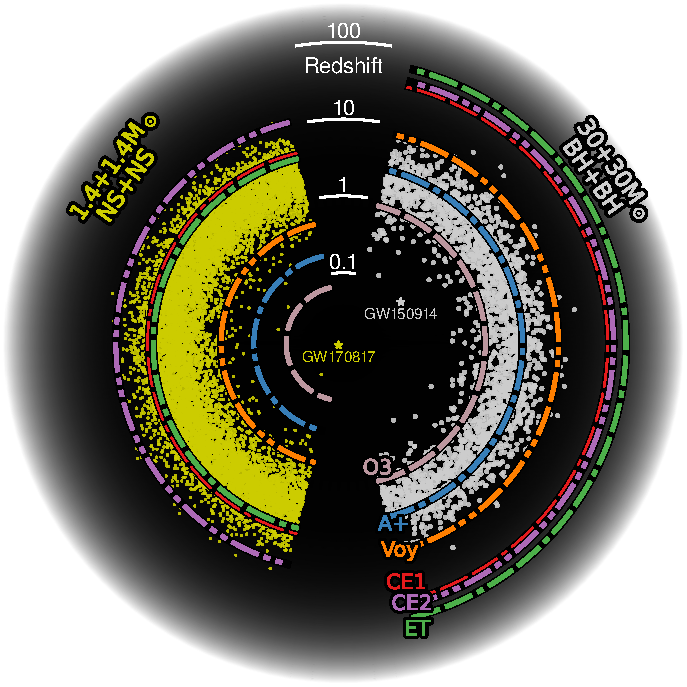
\includegraphics[width=0.9\textwidth]{Figures/horizon_donut_nsns_bhbh_o3_aplus_voy_ce1_ce2_et_redshift.pdf}
    \caption{
Astrophysical range for compact binary systems. The dotted lines show the detection horizons for the different detectors. The detection horizon is the farthest distance to which an optimally oriented source can be seen.
The yellow and white dots are for a simulated population of binary neutron star mergers and binary black hole mergers respectively. Note that beyond z$\sim$6, i.e. in the Dark Ages of the Universe, no sources are shown.
\hspace{\textwidth}
Graphics kindly provided by E.\,Hall (MIT)}
\label{fig:2G-3G_range}
\end{figure}

\begin{figure}[!ht]
    \centering
    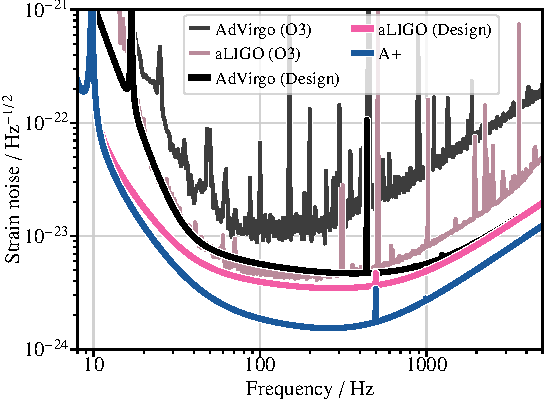
\includegraphics[width=0.7\textwidth]{Figures/advirgoO3_aligoO3_advirgo_aligo_aplus.pdf}
   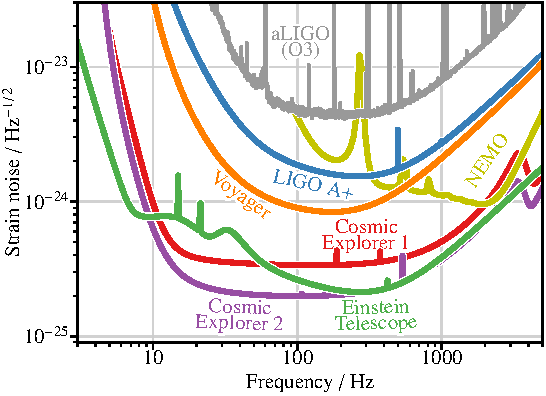
\includegraphics[width=0.7\textwidth]{Figures/aligoO3_aplus_voy_ce1_ce2_et_nemo.pdf}
    \caption{
    The strain sensitivity of various second and third generation detectors, plotted as an amplitude spectrum of detector noise as a function of the frequency. 
    % :\hspace{\textwidth}
    Above -- The second generation and just beyond: Advanced Virgo~(dark grey) and advanced LIGO~(silver pink) in O3, the design of adVirgo~(black) and aLIGO~(pink), and the A+ upgrades (blue). 
    % \hspace{\textwidth}
    Below -- The ``2.5th" and 3rd generation:  
    % \hspace{\textwidth}
    LIGO Voyager~(orange), The first stage of Cosmic Explorer~(red), the second stage of Cosmic Explorer~(purple), the Einstein Telescope~(green) and the Australian detector NEMO~(olive), with Advanced LIGO~(light grey) and The A+ upgrade~(blue) repeated from above for comparison. Shown are the sensitivity curves for sources directly overhead, circularly polarised.
\hspace{\textwidth}
Graphics kindly provided by E.\,Hall (MIT)}
\label{fig:2G-3G_curves}
\end{figure}

When GW detectors gain another order of magnitude in sensitivity we intend to call it a new generation. The first generation was initial LIGO, Virgo, GEO600 and TAMA300. After upgrading to advanced LIGO (aLIGO), advanced Virgo (adVirgo) and newly constructing the underground KAGRA detector we call it the second generation. The current detectors have not yet fully reached their design sensitivity (see figure~\ref{fig:2G-3G_curves}), as some of the last upgrade steps are still pending, such as signal recycling for advanced Virgo, or design parameters have not yet been fully reached, such as the used laser power for advanced LIGO. On the other hand, however, techniques that go beyond the design features of the second generation are already being applied, e.g. squeezed light, as it has demonstrated excellent performance in the smaller gravitational wave detector GEO\,600. The short-term development roadmap with observation objectives and sensitivity progress of the network of currently active GW detectors is described in~\cite{ObservingScenarios}.
Such innovations and technological advances will make it possible to further increase the detectors' sensitivity by a factor of about three before the constraints of the infrastructures prevent any further progress. This intermediate generation between the ``advanced''detectors and the third generation, is usually called ``A+'', i.e. the ``Plus'' version of the advanced detectors~\cite{VirgoAPlus,LIGOA+}. Already for the next observation run O4 some technologies will be employed to reduce quantum noise: 
\begin{itemize}
    \item Currently squeezed light only improves the shot-noise limited frequency range of the detectors, and actually enhances radiation pressure noise at lower frequencies. Optical resonators, so called Filter Cavities, will be installed for frequency-dependent filtering of the squeezed light, which will improve the sensitivity in the high as well as in the low frequency range.
    \item The mass of the mirrors will be increased in Virgo in order to minimise the light's back-reaction on the mirrors and thus reduce the so-called radiant pressure noise. 
    \item The laser power used in the interferometers will be increased as much as thermal deformations caused by point-like absorbing spots on the mirror surfaces and radiation pressure induced effects allow. 
\end{itemize} 

Likely after O4, the mirror coatings will be upgraded, mainly by improving the thermo-mechanical properties of the high reflectivity coatings of the Fabry-Perot cavity mirrors according to the latest research advances. Seismic isolation and mirror suspensions are also on the list of desired improvements.

Until now, interferometers have been operated at room temperature, but their sensitivity is increasingly limited by thermal noise, an effect which as the name suggests has to do with temperature.  One way of reducing this noise is therefore to lower the temperature.  At lower temperatures, however, fused silica as it is currently used in LIGO and Virgo is no longer suitable due to high mechanical loss and the resulting thermal noise such that a different mirror material must be chosen. KAGRA, already pioneering the path of cryogenic interferometers, uses sapphire mirrors. Another promising option is silicon mirrors. This, however, requires a transition to longer laser wavelengths as it is not transparent at the current laser wavelength of 1064\,nm.  Promising candidates are 1550\,nm, a wavelength that is widely used in telecommunications, or \(2\,\mu\)m, where optical absorption is even lower.  The challenge of combining high laser power with the operation of cryogenic optics in combination with the emergent problems of point absorbers, which then tend to cause unacceptable mirror deformations due to local heating, led to the concept of "Voyager"~\cite{Voyager2018}. According to this proposal, an interferometer, operating at a temperature of 123\,K, a laser wavelength of about \(2\,\mu\)m and heavy silicon mirrors, is to be installed in the LIGO infrastructure. This technological concept is also being discussed for the second stage of Cosmic Explorer (see next section).

Another concept that goes beyond the second generation is being developed by Australian researchers. A proposal for a new gravitational wave detector, NEMO (Neutron Star Extreme Matter Observatory)~\cite{NEMO}, abandons high sensitivity in the low-frequency range for cost reasons and concentrates on the frequency range around a few kilohertz. This frequency range is particularly suited for studying the nature of neutron stars. 
The key design aspects of NEMO are the usage of high light power in the interferometer, recycling techniques optimised for high frequencies and the heavy use of squeezed states.
A suitable location on the Australian continent has yet to be found. 

The 3rd generation GW observatories will start operation, at earliest, in the first half of the 2030s. 
In the meantime the existing detectors will be upgraded, while new ones will be built. The Voyager project is one of the options under evaluation, exploring the possibility to anticipate some of the 3rd generation cryogenic technologies in the LIGO detectors.
Based on experience with the current detectors, we anticipate that the biggest challenge in reaching the target low frequency sensitivity for 3G detectors (set by suspension thermal noise, seismic noise, and Newtonian noise {\color{green} (see also chapter 2)}) will be to reduce the multitude of technical noises (such as light scattering and control noises) that can afflict the interferometers. 
% Extending the frequency range of gravitational wave detectors to lower frequencies requires very large detectors like Cosmic Explorer or even underground detectors like in the Einstein Telescope.

The sensitivities of the instruments from the current state to the third generation is shown in Figure~\ref{fig:2G-3G_curves}. 

\section{Cosmic Explorer (CE)}

\subsection{A Brief History of CE}

The first intellectual steps toward the project now known as Cosmic Explorer grew out of efforts within the LIGO Scientific Collaboration (LSC) to conceptualize future gravitational-wave detectors. Devised in the form of a challenge, three teams of scientists, code-named Red, Green, and Blue, developed concepts with differing technological centerpieces. At the conclusion of this process, a conglomerate team with the code-name Lavendar presented a fourth concept, a detector much like Advanced LIGO, only significantly longer. The details of this were further worked out by a team involving members from  MIT and Syracuse University. The last presentation of the GWADW2013 on Elba on 24 May 2013 summarised the vision of this team for a ``Long Uncomplicated Next-Generation Gravitational-Wave Observatory (LUNGO)''\cite{LUNGO}. By 2015, this project became known by the name ``Cosmic Explorer'', which comes from David McClelland of the Australian National University and represents the project's goal to explore the Universe with gravitational waves on cosmological scales. 3G science and research in the US has mostly been carried out within the LSC. 

In 2017, many of the technical noise sources of Cosmic Explorer were worked out, including evaluations of how those noise sources scale with arm length. Detector options with room temperature fused silica test masses (current technology) or cryogenic silicon test masses were considered and noise curves were presented that accounted for optimistic and pessimistic progress by the community on technological research and development~\cite{CE2017}. The project's first dedicated federal funding was awarded the following year through a National Science Foundation award [\# 1836814] as a collaborative grant to five US institutions to study the science case for an international network of next-generation gravitational-wave detectors, and the potential avenues for construction of a 3G detector in the United States. As part of these activities, with members of the LIGO lab, this Cosmic Explorer team wrote and submitted ``Cosmic Explorer: The U.S. Contribution to Gravitational-Wave Astronomy beyond LIGO'', an Astro2020 Decadal Survey APC ground-based technology development white paper, which clarified the timeline and plans for CE~\cite{CE-Astro2020}.

This year (2020), has seen a maturation of the CE concept and the community supporting it. The Cosmic Explorer Consortium was formed in Fall 2020 to provide an open and efficient way for members of the broader physics and astronomy communities to contribute to the conceptualization, design, and future use of CE. Already the consortium has a few hundred members and has begun monthly research and development remote meetings. As a further major step toward building a CE community, the First Cosmic Explorer Meeting, a five-day remote conference, was held in October 2020 with broad community participation to discuss the technical design and the science case for CE. 

\subsection{CE Detector Instrumentation}

Cosmic Explorer is currently envisioned as a single 40-km surface-based facility in the United States with a projected lifetime of 50 years. The CE Horizon Study team, together with the broader community, is however studying alternatives such as multiple CE detectors (such as one in the US and one in Australia) and shorter arm lengths (such as 10, 20, 30\,km) in the context of the achievable science per cost. 

Within this facility, Cosmic Explorer would be built in stages, with upgrades similar to what was done for initial LIGO, enhanced LIGO, Advanced LIGO, and Advanced LIGO$+$. The sensitivity of Cosmic Explorer, compared with other current and future detectors, is shown in Figure~\ref{fig:2G-3G_curves}. 

The first stage of Cosmic Explorer, CE1, is being developed for operations in the 2030s as a relatively low risk first interferometer that would use proven Advanced LIGO$+$ technology, but scaled up to fit the 40\,km baseline facility, to achieve roughly an order of magnitude sensitivity improvement over Advanced LIGO. The optical layout would be that of current interferometers, an L-shaped dual-recycled-Fabry-Perot Michelson Interferometer (DRFPMI), using 1064\,nm wavelength laser light, room temperature fused silica optics, and quadruple pendulum suspensions from active and passive seismic isolation systems. Current studies
%~\cite{CELF} 
anticipate that CE1 will use suspensions similar to LIGO but scaled up and modified to reduce thermal, seismic, and control noises,
% fused silica blade springs attached to the penultimate masses
1.5\,MW of circulating power, 6\,dB of frequency dependent squeezing, and improved inertial sensors for its active seismic isolation. 

The second stage of Cosmic Explorer, CE2, which could operate in the 2040s, could be achieved by a similar room-temperature fused silica interferometer, but with increased Newtonian noise subtraction, even more sensitive inertial sensors, and 10\,dB of frequency dependent squeezing. Or, it could build off of the Voyager technology~\cite{Voyager2018} being developed for a possible upgrade to the existing LIGO facilities using cryogenic silicon optics, 2 micron lasers, and lower-loss optical coatings. Should CE2 use Voyager technology, it would capitalize on the experience with its implementation in LIGO and again primarily scale up the optics and suspensions to match the 40\,km arms and larger facilities. 

Ideas for stages beyond CE2 have not yet been thoroughly developed; they will rest upon research and development breakthroughs in the coming decades. For this reason, the CE facility will be built with enough room and flexibility to allow moving of vacuum chambers and other equipment to accommodate different configurations (take for instance the current work happening for Advanced LIGO$+$ where vacuum tanks and tubes are being added to realize 300\,m quantum noise filter cavities -- a technology that was not yet mature when Advanced LIGO was proposed).

\subsection{CE Status and Timing}

The current focus for Cosmic Explorer is on drafting and soliciting feedback on a ``Horizon Study'' whitepaper detailing the scientific goals and capabilities and the design and management considerations for CE. Current activities toward this study include: a ``trade study" aimed at evaluating how well the science goals of CE can be met by various detector configurations and global networks; the development of a reference design and an associated cost-schedule estimate for the construction of CE; the identification of land large enough to host a CE detector while minimizing earth moving costs; civil engineering costing for three reference sites that will be parameterized to estimate project costs at other candidate locations; investigation of novel and low-cost vacuum systems for the long arms; and a more detailed evaluation of the noise sources that will limit CE's performance. A whitepaper, strengthened by these studies, will be delivered in 2021 to the scientific community through various forums for feedback and further contributions. In parallel, possible funding avenues for CE are being investigated. 

\section{Einstein Telescope (ET)}
\subsection{A Brief History of ET}
% Michele
The idea of a $3^{rd}$ generation (3G) GW observatory was elaborated for the first time in 2004 by a working group studying the future of GW detectors in the European project ILIAS (2004-2008), funded by the European Commission in the $6^{th}$ Framework Programme (FP6). An exploratory workshop was funded by the European Science Foundation (ESF) in 2005, where the basis of the Einstein Telescope proposal was set. The name "Einstein Telescope" and its short form ``ET'', which nicely hints at the exclusively extraterrestrial origin of our signals, was selected in March 2007, after a long debate considering a wide variety of (sometimes most peculiar) names and acronyms. 

The first crucial step for the Einstein Telescope project was the approval and then funding of the ET conceptual design study proposal by the European Commission within the $7^{th}$ Framework Programme (FP7). The Conceptual Design Report (CDR) for the ET project was delivered in 2011~\cite{ET-CDR}; the CDR elaborates the concept of Research Infrastructures or Observatory, focusing the attention on the infrastructure to be designed and realised for ET with the capability to allow future upgrades of the hosted detectors for decades. 
The following years, mainly dedicated to the upgrades, operation and data analysis of the $2^{nd}$ generation GW detectors, Advanced Virgo and Advanced LIGO, allowed the ET scientific community to grow, the "3G idea" to spread and some of the basic technologies to be developed through a series of small grants in Europe.

The second crucial step for the ET project was taken in September 2020.  
An alliance of five national governments (Belgium, Poland, Spain and the Netherlands, led by Italy) and a consortium of 41 institutions, including some from Germany, Hungary, Norway, Switzerland and the United Kingdom, proposed to include ET in the 2021 update of the ESFRI~\cite{ESFRI} roadmap, which describes the major European research infrastructures to be built in the decade 2021--2030. A large part of the description of ET in this chapter is based on the documentation of the ESFRI proposal. 

\subsection{ET Detector Instrumentation}
The Einstein Telescope will be a new gravitational wave observatory with a unique design as detailed in the "Einstein Telescope: Science Case, Design Study and Feasibility Report"~\cite{ET_Update}.
ET will improve the sensitivity by an order of magnitude with respect to the design sensitivity of Advanced Virgo and Advanced LIGO and extend the observation band towards lower frequencies, i.e. down to about 3\,Hz compared to $\sim 10$\,Hz for the advanced Virgo and advanced LIGO design.
Its design combines the proven concepts from current detectors, i.e. a
modified Michelson interferometer, with Fabry-Perot cavities in the arms and power recycling and signal recycling techniques with advanced upgrades in an ultra-low-noise infrastructure designed to accommodate several technology upgrades over a period of 50 years.
\begin{figure}[ht]
  \begin{minipage}[t]{0.43\textwidth}
  \vspace{0pt}\hspace{8mm}
    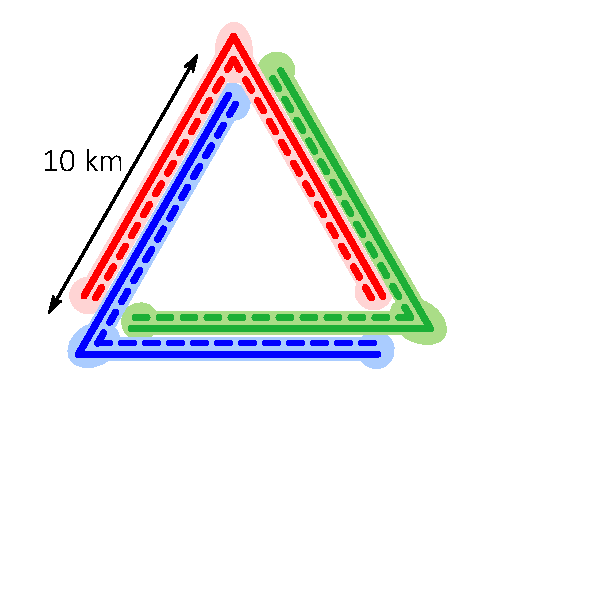
\includegraphics[width=\textwidth]{Figures/ET_simpleB.pdf}
  \end{minipage}\hfill
  \begin{minipage}[t]{0.45\textwidth}
    \caption{
       The Einstein Telescope will consist of three nested detectors (shown in blue, green and red) in a triangular arrangement. Each detector consists of two interferometers, one optimised for low-frequency (solid) and one for high-frequency sensitivity (dashed).
    } \label{fig:NestedDetectors}
  \end{minipage}\hspace{5mm}
 \end{figure}


%(taken from the 30 pages document in only slightly modified form)\\

\noindent Specific ET design concepts are: 

\textbf{\textit{Triangle}}\quad ET will consist of three nested detectors in a configuration of an equilateral triangle, pair-wise sharing a 10\,km long tunnel, resulting in an angle between the detector arms of $60\,^\circ$. With a minimum of tunnelling, this configuration will enable ET to resolve the GW polarization, provide a null stream  and allow for continuous operation during maintenance.

\textbf{\textit{10\,km}}\quad The ET detectors will have 10\,km long arms, to increase the signals produced by the GWs compared to current detectors and thereby reducing the impact of virtually all of the sensitivity-limiting noise sources.
  
\textbf{\textit{Xylophone}}\quad 
Each of the three ET detectors will be composed of a pair of complementary interferometers, one with a peak sensitivity at low frequencies and the other with a sensitivity optimised for higher frequencies. 
The reason is to separate the challenges related to the use of high power stored in the arms (needed to reduce the photon shot noise) such as thermal and radiation pressure effects, from those related to achieving the targeted low-frequency sensitivity (limited by Brownian noise, quantum back-action noise and radiation pressure driven control noise).\\
The high power detector (3\,MW) \textbf{\textit{ET-HF}}, operating at room temperature, covers the high frequency range ($>$\,35\,Hz) and largely uses today's advanced detector technology, pushing it to its physical and technical limits.\\
The low power detector \textbf{\textit{ET-LF}}, which operates at a temperature of 10-20\,K and a low power of circulating light (18\,kW), is optimised for low frequency ($<$\,35\,Hz) gravitational wave sources. Operation at cryogenic temperatures requires a new material for the mirrors because the mechanical properties of fused silica, as used in current detectors, deteriorate at cryogenic temperatures. Silicon will therefore be used as mirror material, which causes a change of the laser wavelength to about 1550\,nm.\\
\textbf{\textit{Underground operation}}\quad By building the Einstein telescope underground at a depth of 200\,-\,300\,m, the influence of seismic waves and compression waves of the surrounding air is reduced, thus minimizing seismic and Newtonian noise.
This allows an extension of the sensitivity range of ET down to a few Hertz. 
The three 10\,km long tunnels, each with an internal diameter of 6.5\,m and containing four vacuum tubes, as well as the caverns with the large vacuum tanks are being excavated using well-established tunnelling and underground construction techniques. 
In addition to the main caverns at the vertices of the triangle, several auxiliary caverns will host further interferometer components. \\
The design sensitivity curve is shown in fig.~\ref{fig:ET_sensitivity}.

\begin{figure}[!h]
	\centering
		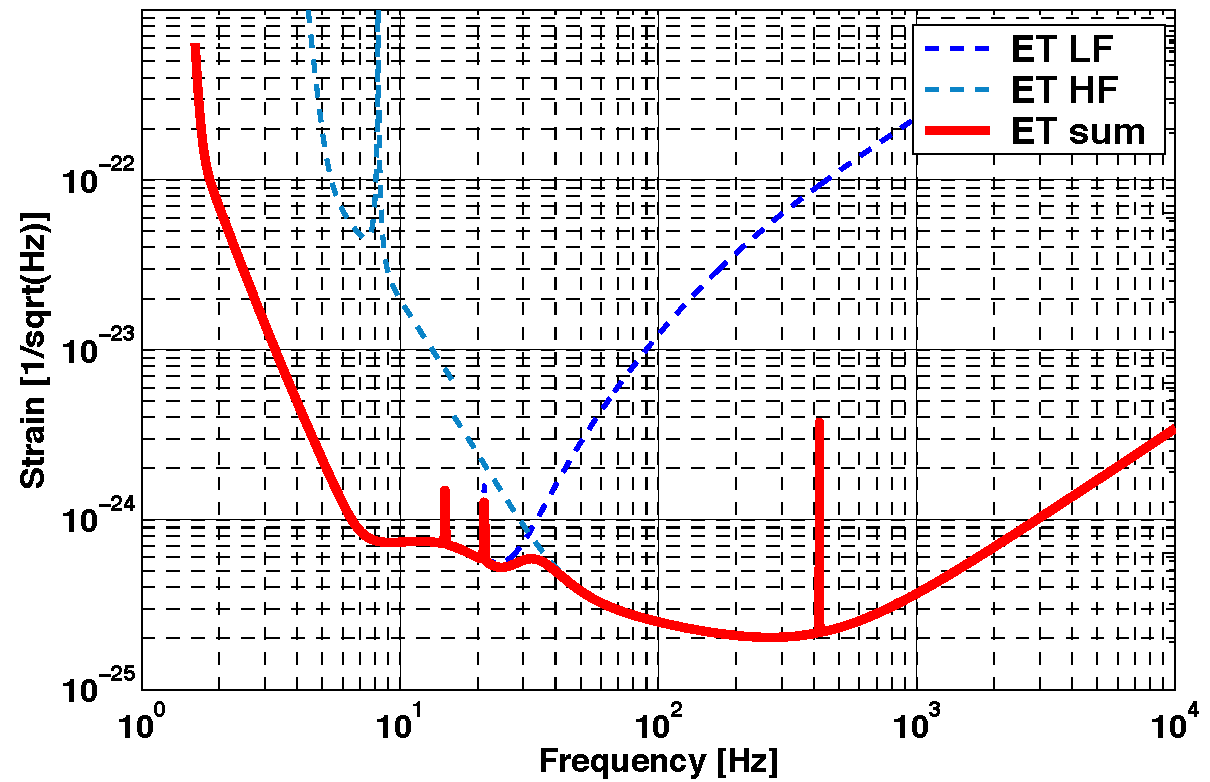
\includegraphics[width=0.9\textwidth]{Figures/ET_2020_spectrumtriangle.pdf}
	\caption{Sensitivity of the Einstein Telescope in the `xylophone' configuration. 
	The sensitivity of the low-frequency cryogenic interferometer is shown in the  dashed dark blue curve and the one of the high-frequency room temperature	one in a dashed blue-green tone. The sum of both is given by the solid bright red curve. Shown is the sensitivity for sources directly overhead, circularly polarised.}
	\label{fig:ET_sensitivity}
\end{figure}

\subsection{ET Status and Timing}
At the moment of writing (end 2020) the Einstein Telescope has been proposed for inclusion in the update of the ESFRI (European Strategy Forum for Research Infrastructures) roadmap. There are two site candidates - one on the Italian island of Sardinia and the other in the province of Limburg in the south-east of the Netherlands. Site selection is expected around 2024. Depending on funding availability, building the infrastructure could start as early as 2027 and will take 6-8 years. The installation of the three detectors in the infrastructure will follow in a staged way one by one such that the Einstein Telescope can give first data in the mid-late 30's.

\section{Down Under} %need a better title?
A network of third generation gravitational wave detectors would greatly benefit from an additional facility in Australia. Located in the southern hemisphere, such a site in addition to sites in Europe and the USA, would be ideal as it maximises the area of the enclosed triangle, thereby improving the trilateration to determine the direction of the source.
This improved pointing accuracy from another gravitational wave detector in Australia has also been valid for the second generation, i.e. advanced LIGO and advanced Virgo and hence efforts have been made shortly after the turn of the millennium to move one of the three initial LIGO detectors to Australia. However, these plans failed due to funding difficulties, and a third LIGO detector is now being built in India. The possibility of building a second CE site in Australia is being actively studied.

\section{The Path to 3G Observatories}
Some of the technologies for the third generation of gravitational wave detectors are already well developed and are expected to evolve to a level required for the third generation during the A+ upgrades of the advanced detectors, such as squeezed light and lasers for 1064\,nm and 1550\,nm or auxiliary optics. Also vacuum technology is mature enough so that the vacuum systems required could be built with today's technology, but 3G designers are hoping to make considerable savings with innovative techniques, especially in cost-intensive subsystems. 
A small selection of the many research and development topics needed to make 3G detectors a reality are the following:
The cryo-technology to cool mirrors to the desired temperature is basically available, but bringing the necessary cooling power to the mirrors without short circuiting the seismic isolation is a significant challenge. Developing coatings with superb optical quality and substantially reduced thermal noise at room temperature and cryogenic temperatures is one of the most prominent challenges. Further development of 2\,$\mu$m quantum noise technology must be done. In order to achieve adequate optical performance at the new wavelengths of 1550\,nm or 2\,$\mu$m, large ultrahigh purity substrates weighing 200-300\,kg are required, and have to be polished to extreme specifications. 
\\

Gravitational wave science is an extremely active research field with the promise of revolutionary scientific discoveries in the coming decades. Now is the time to forge ahead with the construction of the next generation of GW observatories. 

%%%%%%%%%%%%%%%%%%%%%%%% reference.tex %%%%%%%%%%%%%%%%%%%%%
% sample references
% 
% Use this file as a template for your own input.
%
%%%%%%%%%%%%%%%%%%%%%%%% Springer%%%%%%%%%%%%%%%%%%%%%%%%%%
%
% BibTeX users please use
% \bibliographystyle{}
% \bibliography{}
%
\begin{thebibliography}{99.}
% Book Chapter
\bibitem{basic-contrib} Brown B, Aaron M (2001) The politics of nature. In: Smith J (ed) The rise of modern genomics, 3rd edn. Wiley, New York, p 234--295  
%
% Online Document
\bibitem{basic-online} Dod J (1999) Effective Substances. In: The dictionary of substances and their effects. Royal Society of Chemistry. Available via DIALOG. \\
\url{http://www.rsc.org/dose/title of subordinate document. Cited 15 Jan 1999}
%
% Journal article by DOI
\bibitem{basic-DOI} Slifka MK, Whitton JL (2000) Clinical implications of dysregulated cytokine production. J Mol Med, doi: 10.1007/s001090000086
%
% Journal article
\bibitem{basic-journal} Smith J, Jones M Jr, Houghton L et al (1999) Future of health insurance. N Engl J Med 965:325--329
%
% Monograph
\bibitem{basic-mono} South J, Blass B (2001) The future of modern genomics. Blackwell, London 
%
\end{thebibliography}
\end{document}